
\documentclass{article}
\usepackage[utf8]{inputenc}
\usepackage[T1]{fontenc}
\usepackage[frenchb]{babel}
\usepackage[bookmarks=true]{hyperref}
\usepackage{lmodern}
\usepackage{graphicx}


\author{Gentile Pierre, Didier-Roche François}
\date{\today}
\title{Document de conception générale}

\frenchbsetup{StandardLists=true}

\begin{document}

\maketitle

\newpage
\tableofcontents
\newpage


\section{Introduction}
\subsection{Objet et portée du document}
Ce document décrit de façon générale comment est construite l'application Appointime. Il s'adresse particulièrement
 aux personnes souhaitant connaître l'architecture générale de l'application sans entrer dans les details.


\subsection{Références}



\subsection{Vue d'ensemble}
Dans la suite du document, nous verrons dans un premier temps quels sont les acteurs et comment peuvent-ils agir 
sur le système. Nous verrons ensuite via des diagrammes de cas d'utilisation 
tous les cas d'utilisation qu'offre l'application Appointime. Ensuite, nous présenterons les classes
 principales que va utiliser l'application et les relations entre celles-ci. Enfin, nous verrons comment sera gérée la persistance des données.


\section{Cas d'utilisation}
\subsection{Acteurs}
\subsubsection{Utilisateur dit "particulier"}
Un utilisateur dit "particulier" est un utilisateur recherchant un service proposé par un utilisateur dit "professionnel".
Ces utilisateurs constituent la majorité des usagers de l'application.
Il n'auront pas la possibilité de
\begin{itemize}
  \item proposer des services,
  \item d'avoir un calendrier de rendez-vous,
  \item d'avoir une entrteprise.
\end{itemize}
Ils auront la possibilité de
\begin{itemize}
  \item rechercher des services et/ou des professionnels,
  \item prendre un rendez-vous pour un service,
  \item de payer directement certains professionnels via l'application,
  \item d'accéder à la gestion de leur compte.
\end{itemize}


\subsubsection{Utilisateur dit "professionnel"}
Un utilisateur dit "professionnel" est un utilisateur proposant un ou plusieurs services aux autres utilisateurs.
Ces utilisateurs constituent la minorité des usagers de l'application.
Un utilisateur dit "professionnel" aura la possibilité de
\begin{itemize}
  \item proposer des services,
  \item gérer des services,
  \item d'avoir un calendrier de rendez-vous,
  \item gérer son calendrier de rendez-vous,
  \item d'avoir une entreprise,
  \item gérer son entreprise (description, horaires).
  \item profiter des mêmes services que les utilisateurs dit "particuliers".
\end{itemize}


\subsection{Liste et diagrammes de cas d'utilisation}
\subsubsection{Inscription}
Ce cas permet de s'inscrire sur l'application en tant que particulier ou professionnel.
Dans le cas d'un professionnel, ce dernier pourra ensuite profiter des droits qui lui sont accordés.

\begin{center}
  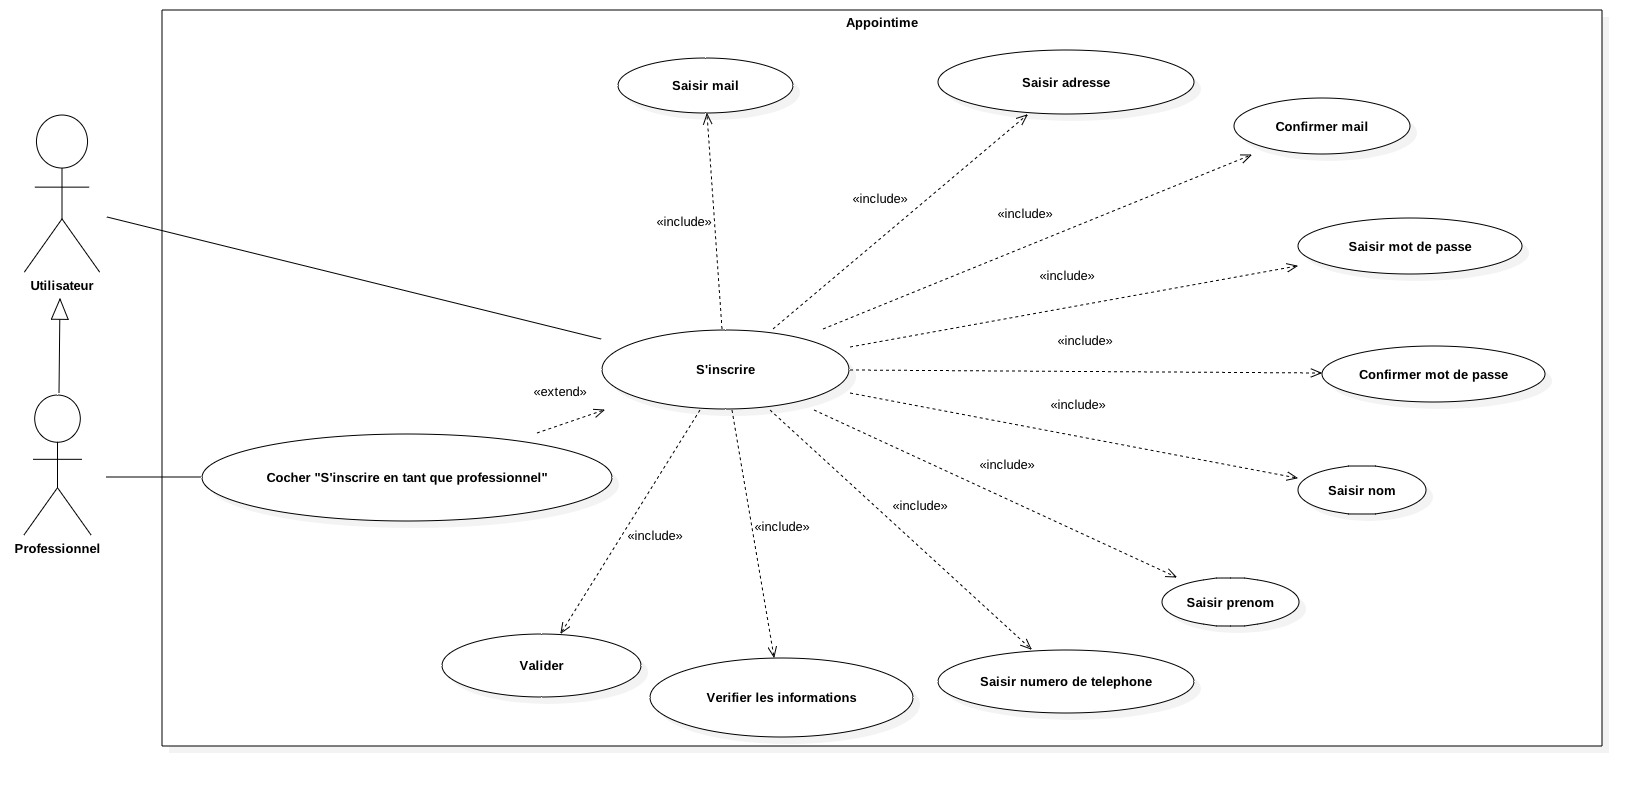
\includegraphics[width=350pt]{diagram/useCaseInsc}
\end{center}


\subsubsection{Gestion de compte}
Ce cas permet de modifier ses informations.
\begin{center}
  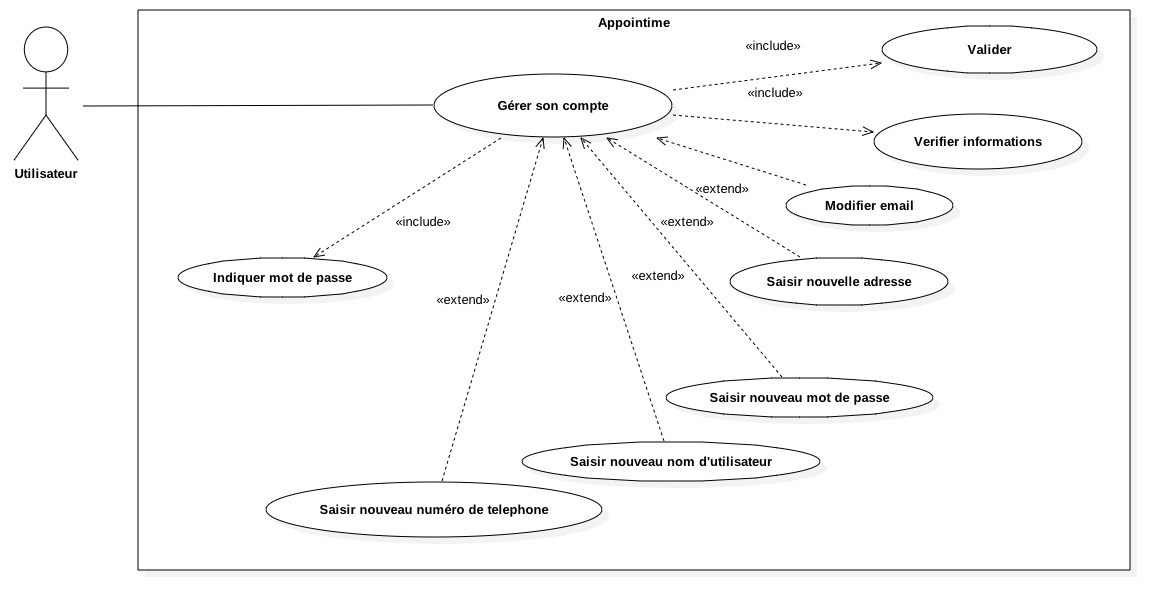
\includegraphics[width=350pt]{diagram/useCaseGererCompte}
\end{center}

\subsubsection{Connexion}
Ce cas permet de se connecter à l'application.
\begin{center}
  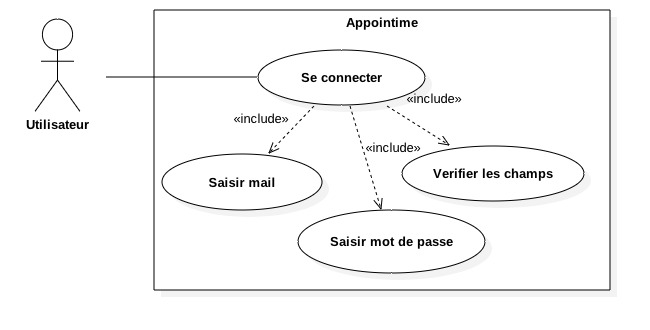
\includegraphics[width=350pt]{diagram/useCaseConnexion}
\end{center}

\subsubsection{Création d'une entreprise}
Ce cas permet à un professionnel de créer son entreprise et de renseigner les informations relatives à celle-ci après son inscription.
\begin{center}
  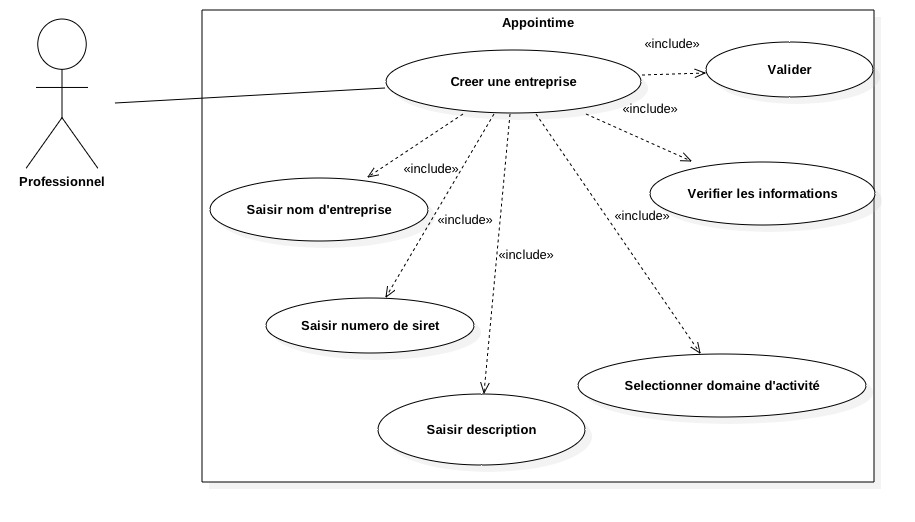
\includegraphics[width=350pt]{diagram/useCaseCreerEntreprise}
\end{center}


\subsubsection{Recherche de professionnel}
Ce cas permet à un utilisateur de rechercher un professionnel via un nom, un secteur d'activité ou un flashcode.
\begin{center}
  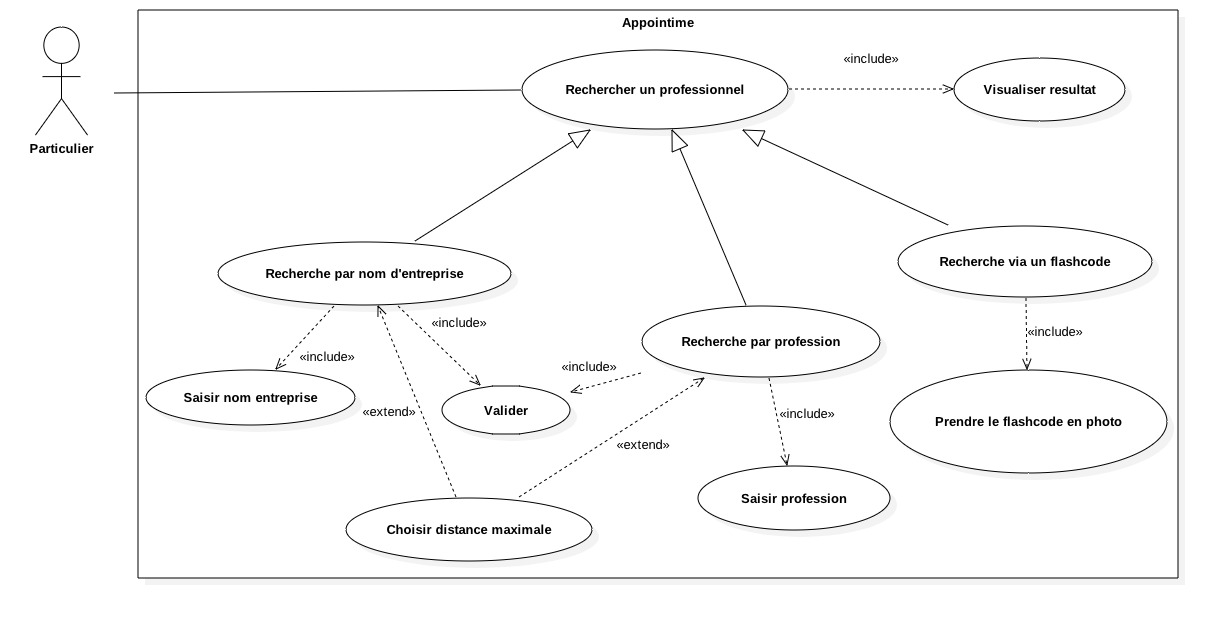
\includegraphics[width=350pt]{diagram/useCaseRecherchePro}
\end{center}

\subsubsection{Gestion des horaires}
Ce cas permet à un professionnel de gérer les horaires d'ouverture de son entreprise.
\begin{center}
  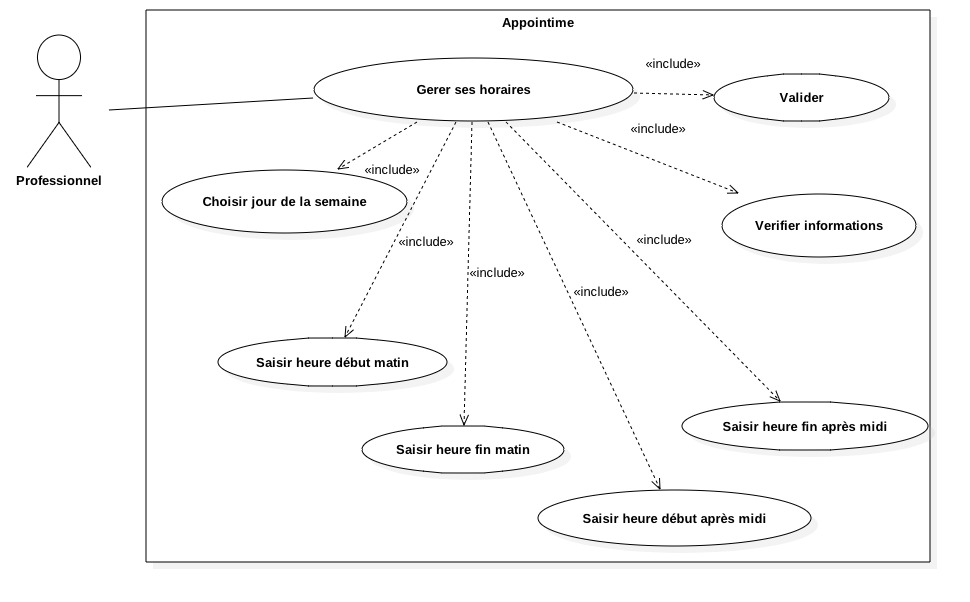
\includegraphics[width=350pt]{diagram/useCaseGererHoraire}
\end{center}

\subsubsection{Création de préstation}
Ce cas permet à un professionnel de créer une prestation.
\begin{center}
  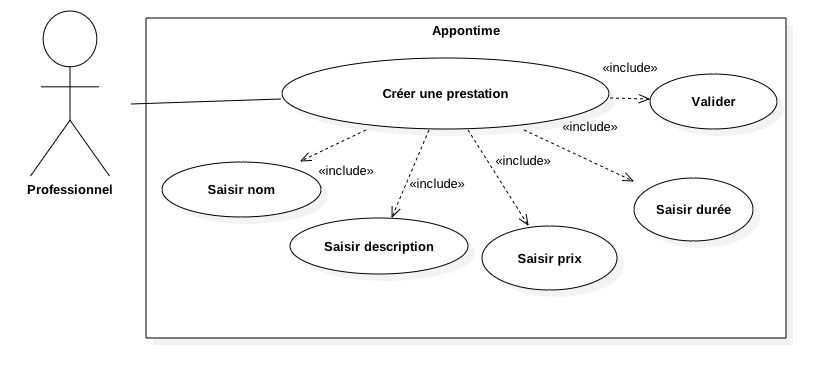
\includegraphics[width=350pt]{diagram/useCaseCreerPrestation}
\end{center}
\subsubsection{Prise de rendez-vous}
Ce cas permet de prendre un rendez-vous chez un professionnel à un horaire libre.
\begin{center}
  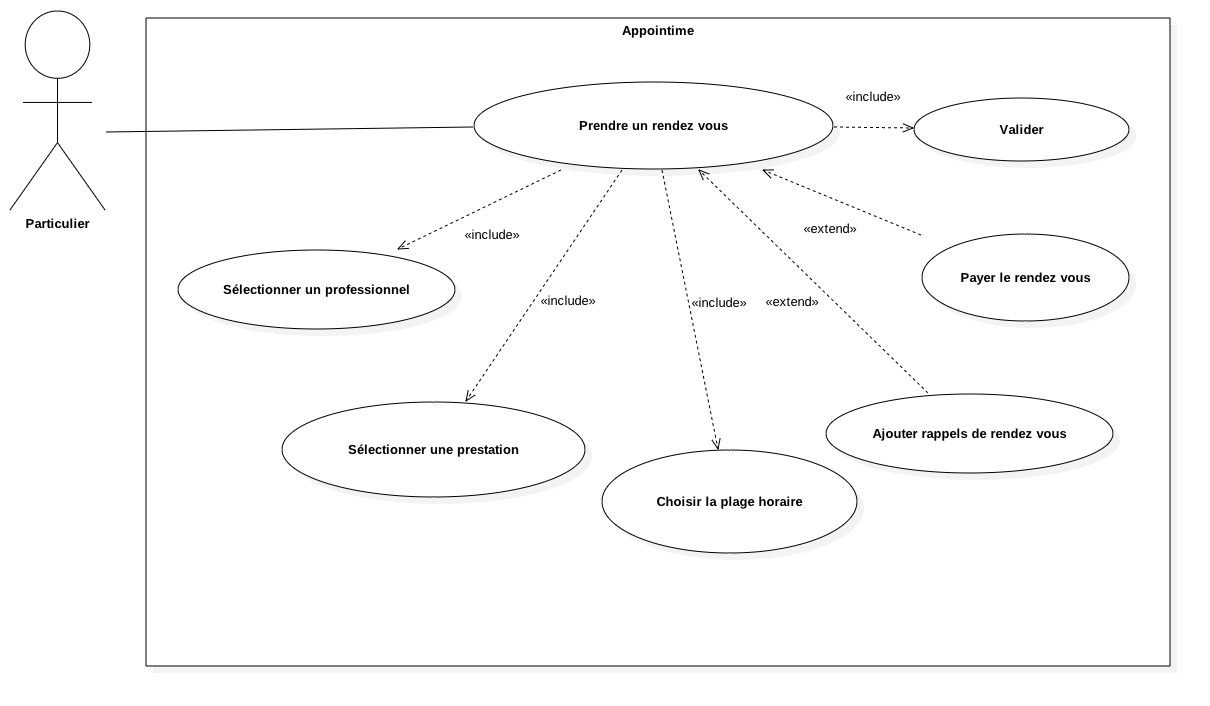
\includegraphics[width=350pt]{diagram/useCasePriseRdv}
\end{center}
\subsubsection{Confirmation de rendez-vous}
Ce cas permet à un professionnel de confirmer ou non un rendez-vous pris préalablement par un particulier.
\begin{center}
  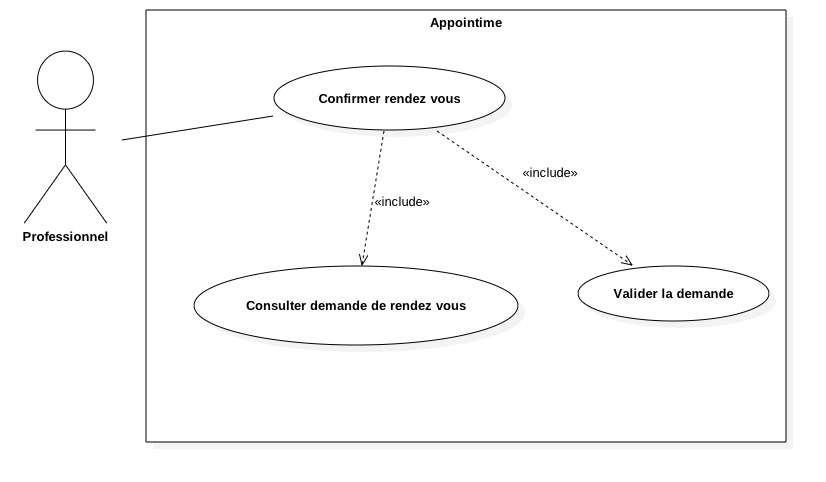
\includegraphics[width=350pt]{diagram/useCaseConfirmerDemande}
\end{center}
\section{Diagrammes d'activité}
\subsection{Inscription}
\begin{center}
  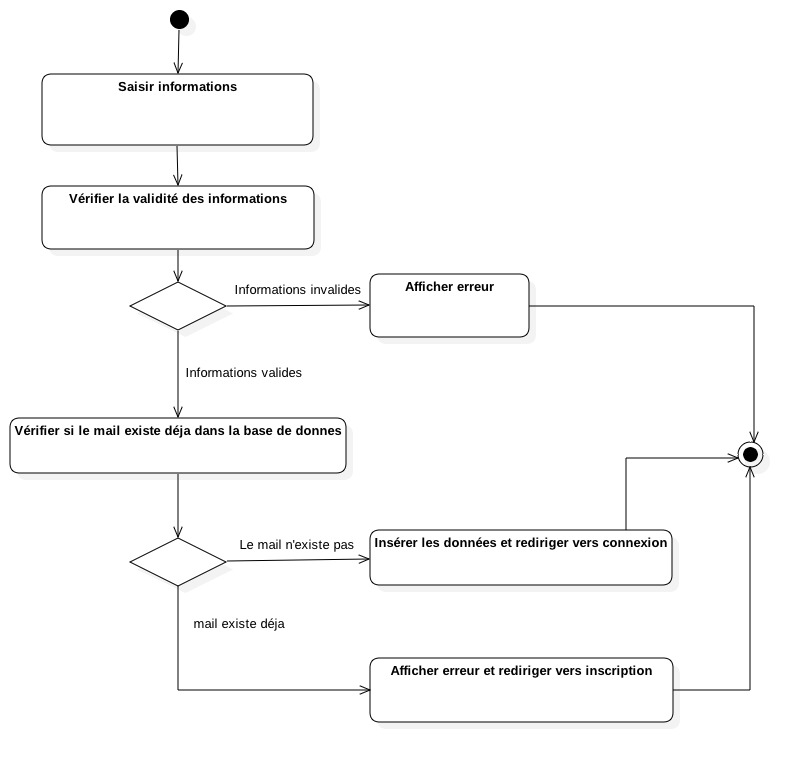
\includegraphics[width=350pt]{diagram/activiteInscription}
\end{center}
\subsection{Connexion}
\begin{center}
  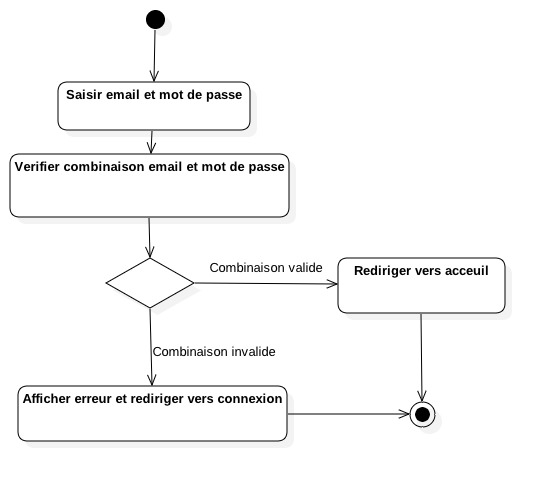
\includegraphics[width=350pt]{diagram/activiteConnexion}
\end{center}
\subsection{Création d'une entreprise}
\begin{center}
  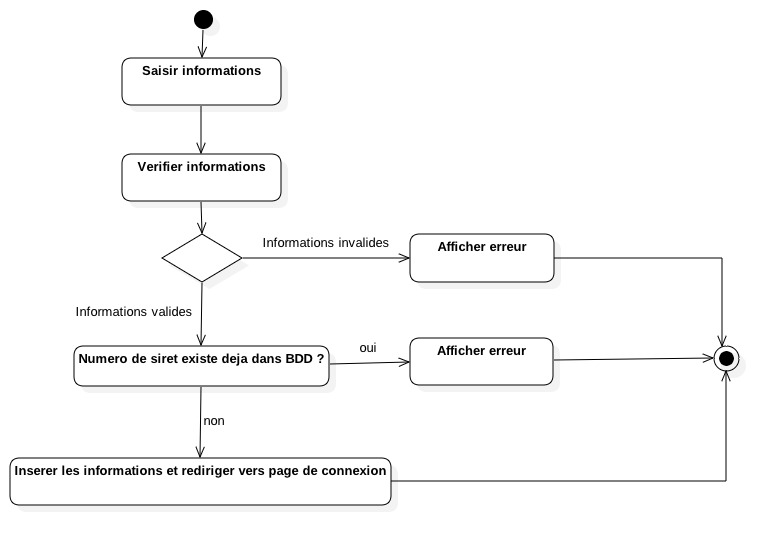
\includegraphics[width=350pt]{diagram/activiteCreerEntreprise}
\end{center}


\section{Description et interaction des classes}
\subsection{Description des classes}
\subsubsection{La classe Utilisateur}
La classe Utilisateur definit les utilisateurs qu'ils soient particuliers ou professionnels. Cette classe est composée des attributs suivants :
\begin{itemize}
\item \textbf{id\_utilisateur} : un identifiant unique représenté par un entier Long,
\item \textbf{email\_utilisateur} : une chaîne de caractères (String) représentant un email unique,
\item \textbf{nom\_utilisateur} : une chaîne de caractères (String) représentant le nom de l'utilisateur,
\item \textbf{prenom\_utilisateur} : une chaîne de caractères (String) représentant le prénom de l'utilisateur,
\item \textbf{pass\_utilisateur} : une chaîne de caractères (String) représentant le mot de passe de l'utilisateur,
\item \textbf{adresse\_utilisateur} : une chaîne de caractères (String) représentant l'addresse de l'utilisateur,
\item \textbf{telephone\_utilisateur} : une chaîne de caractères (String) représentant le numéro de téléphone de l'utilisateur,
\item \textbf{est\_professionnel} : un booleen indiquant si l'utilisateur est un professionnel ou un particulier (1 si professionnel, 0 si particulier),
\item \textbf{points} : un entier indiquant les points restant de l'utilisateur.
\end{itemize}

\subsubsection{La classe Entreprise}
La classe Entreprise décrit une entreprise et est composée d'une liste de calendrier, une liste de prestations et d'un utilisateur (le professionnel lié à cette entreprise) 
Voici la liste de ses attributs :
\begin{itemize}
\item \textbf{id\_entreprise} : un identifiant unique représenté par un entier Long,
\item \textbf{utilisateur} : le professionnel lié à cette entreprise, représenté par un type Utilisateur,
\item \textbf{prestations} : les prestations liées à cette entreprise, représenté par une liste de Prestation,
\item \textbf{calendrier} : le calendrier lié à cette entreprise, représenté par une liste de Calendrier,
\item \textbf{domaine\_activite} : une chaîne de caractères (String) définissant le domaine d'activité de l'entreprise,
\item \textbf{description} : une chaîne de caractères (String) décrivant l'entreprise,
\item \textbf{addresse} : une chaîne de caractères (String) représentant l'adresse de l'entreprise,
\item \textbf{annulation\_rdv} : un entier (int) indiquant la durée minimale avant laquelle un particulier peut annuler un rendez-vous,
\item \textbf{num\_siret} : une chaîne de caractères (String) unique représentant le numéro de siret de l'entreprise.
\end{itemize}

\subsubsection{La classe Calendier}
La classe Calendrier décrit un calendrier et est composée des attributs suivants :
\begin{itemize}
\item \textbf{id\_calendrier} : un identifiant unique représenté par un entier Long,
\item \textbf{demi\_journee} : un entier représentant la demi-journée que definit cette instance de calendrier (par exemple, lundi matin = 1),
\item \textbf{heure\_debut} : une date de type Date représentant l'heure de début de service,
\item \textbf{heure\_fin} : une date de type Date représentant l'heure de fin de service,
\item \textbf{ouvert} : un booleen indiquant si le professionnel propose ses services durant CETTE demi-journée (1 si oui, 0 si non).
\end{itemize}

\subsubsection{La classe Prestation}
\begin{itemize}
\item \textbf{id\_prestation} : un identifiant unique représenté par un entier Long,
\item \textbf{titre\_prestation} : une chaîne de caractères (String) représentant le titre de la prestation,
\item \textbf{description\_prestation} : une chaîne de caractères (String) décrivant la prestation,
\item \textbf{duree\_prestation} : un entier décrivant la durée de la prestation,
\item \textbf{prix\_prestation} : un float représentant le prix de la prestation,
\item \textbf{confirmation\_auto} : un booleen indiquant si lors d'une prise de rendez-vous avec cette prestation, la confirmation est automatique ou non(1 si oui, 0 si non).

\end{itemize}

\subsubsection{La classe RendezVous}
La classe RendezVous est composée d'un utilisateur et d'une entreprise.
Voici la liste de ses attributs :
\begin{itemize}\item 
\textbf{utilisateur} : le particulié lié à ce rendez vous, représenté par un type Utilisateur,
\item \textbf{entreprise} : l'entreprise lié à ce rendez vous, représenté par un type Entreprise,
\item \textbf{id\_rdv} : un identifiant unique représenté par un entier Long,
\item \textbf{heure\_debut} : une date de type Date représentant l'heure de début du rendez-vous,
\item \textbf{heure\_fin} : une date de type Date représentant l'heure de fin du rendez-vous.
\end{itemize}



\subsection{Diagramme de classe}
\begin{center}
  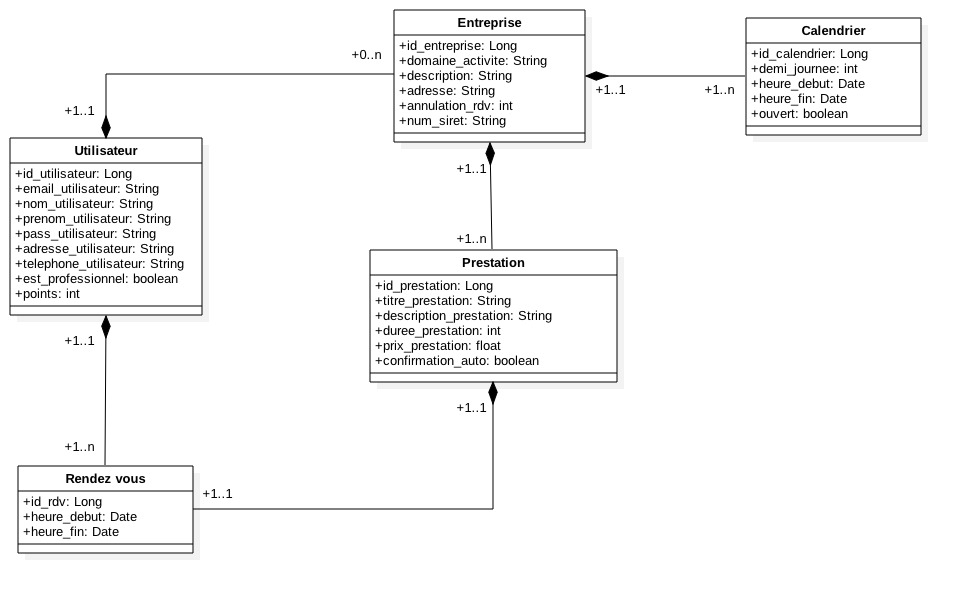
\includegraphics[width=350pt]{diagram/class}
\end{center}


\section{Description de la persistance des données}
\subsection{Outils utilisés}
Pour la persistance des données, nous utiliserons une base de données MySQL decrite plus bas via un modèle entité association.
\subsection{Modèle entité association}
\begin{center}
  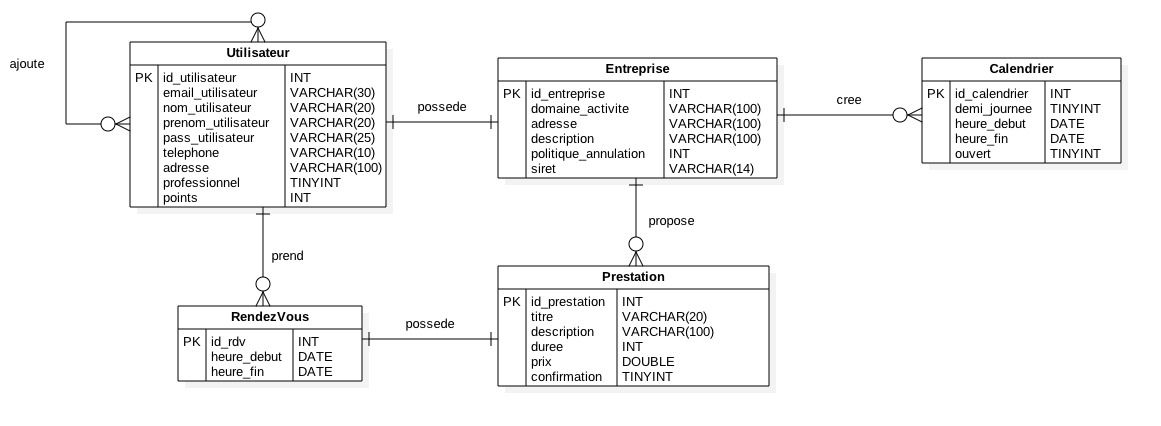
\includegraphics[width=350pt]{diagram/entite}
\end{center}














\end{document}
